% credit: https://github.com/makokal/beamer-themes
\documentclass{beamer}
\usetheme{ALUF}

\usepackage[utf8]{inputenc}
% \usepackage{palatino}
% \usepackage[T1]{fontenc}
\usepackage{lmodern}
\usepackage[expert]{mathdesign}
\usepackage[protrusion=true,expansion=true,tracking=true,kerning=true]{microtype}

\usepackage{algorithm2e}
% \usepackage{multimedia}
\usepackage{media9}
\usepackage{multirow}

\title{Facial emotion recognition with latent topics modeling on local features}
\subtitle{AI project}
\author{Vo Thanh Hung}
\date{June 2019}
% \institute{\url{email@some-cool-place.ext}\\\url{http://www.cool-url.com}}

\graphicspath{ {imgs/} }
\begin{document}

\begin{frame}[plain,t]
\titlepage
\end{frame}

\begin{frame}% [plain,t]
	\frametitle{Outline}
\tableofcontents
\end{frame}

%=============================================================================================

% -----------------------------------
% FER introduction
% -----------------------------------
\section{Introduction}
\begin{frame}{Facial emotion recognition (FER)}

\begin{figure}[h!]
\centering
\begin{tabular}{|c|c|c|c|c|c|c|}
  \hline
  \tiny Surprise & \tiny Fear & \tiny Disgust & \tiny Happiness & \tiny Sadness & \tiny Anger & \tiny Neutral \\
  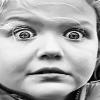
\includegraphics[width=.1\textwidth]{imgs/train_00006_aligned-1.jpg} &
  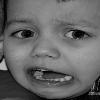
\includegraphics[width=.1\textwidth]{imgs/train_00027_aligned-2.jpg} &
  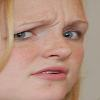
\includegraphics[width=.1\textwidth]{imgs/train_00031_aligned-3.jpg} &
  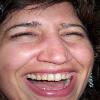
\includegraphics[width=.1\textwidth]{imgs/train_00016_aligned-4.jpg} &
  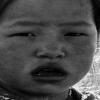
\includegraphics[width=.1\textwidth]{imgs/train_00005_aligned-5.jpg} &
  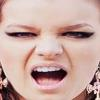
\includegraphics[width=.1\textwidth]{imgs/train_00047_aligned-6.jpg} &
  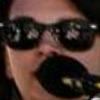
\includegraphics[width=.1\textwidth]{imgs/train_09757_aligned-7.jpg} \\

  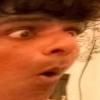
\includegraphics[width=.1\textwidth]{imgs/test_0043_aligned-1-2.jpg} &
  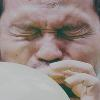
\includegraphics[width=.1\textwidth]{imgs/test_0274_aligned-2-2.jpg} &
  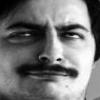
\includegraphics[width=.1\textwidth]{imgs/train_09745_aligned-3-2.jpg} &
  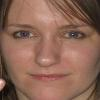
\includegraphics[width=.1\textwidth]{imgs/test_0055_aligned-4-2.jpg} &
  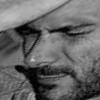
\includegraphics[width=.1\textwidth]{imgs/test_0049_aligned-5-2.jpg} &
  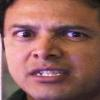
\includegraphics[width=.1\textwidth]{imgs/test_0057_aligned-6-2.jpg} &
  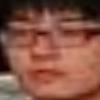
\includegraphics[width=.1\textwidth]{imgs/train_09759_aligned-7-2.jpg} \\
  \hline
\end{tabular}
\caption{Images from RAF-DB}
\label{fig:raf-db-example}
\end{figure}

\end{frame}

\begin{frame}{Project objective}
    \begin{itemize}
        \item<1-> FER problem
        \item<2-> Basic emotion
        \item<3-> Dataset: RAF-DB
        \item<4-> Feature extractor: SIFT, SUFT, KAZE
        \item<5-> Method: Bag-of-Words, HDP
        \item<6-> Classifier: SVM, NB and RF
    \end{itemize}
\end{frame}

\section{Related work}
\begin{frame}{Image feature extraction}
    \begin{itemize}
        \item<1-> SIFT
        \item<2-> SUFT
        \item<3-> KAZE
        \item<4-> etc.
    \end{itemize}
\end{frame}

\begin{frame}{Bag-of-Words}
    \begin{itemize}
        \item Three groups of features are clustering and build vocabulary
        \item Image features are converted to vector
        \item TF-IDF is used to make vector
    \end{itemize}
\end{frame}

\begin{frame}{Latent topics modeling}
    \begin{itemize}
        \item<1-> Latent Dirichlet Allocation (LDA)
        \item<2-> Hierarchical Dirichlet process (HDP)
    \end{itemize}
    
    \begin{figure}
        % \centering
        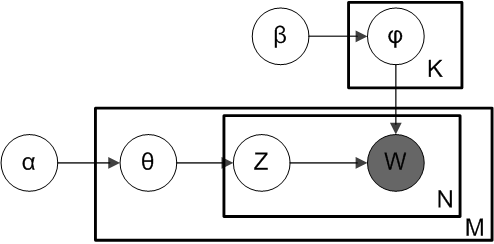
\includegraphics[width=.5\textwidth]{Latent_Dirichlet_allocation-1.png}
        \caption{LDA} \label{fig:LDA}
    \end{figure}
    
    {\tiny
    $\alpha$ is the parameter of the Dirichlet prior on the per-document topic distributions \\
    $\beta$ is the parameter of the Dirichlet prior on the per-topic word distribution \\
$\theta _{i}$ is the topic distribution for document $i$ \\
$\varphi _{k}$ is the word distribution for topic $k$ \\
$z_{ij}$ is the topic for the $j^{th}$ word in document $i$ \\
$w_{ij}$ is the specific word \\
}
    \vspace{0.5cm}
    \textit{\tiny (Source: https://en.wikipedia.org/wiki/Latent\_Dirichlet\_allocation)}
\end{frame}

\section{System architect}
\begin{frame}{System architect}
    \begin{figure}
        \centering
        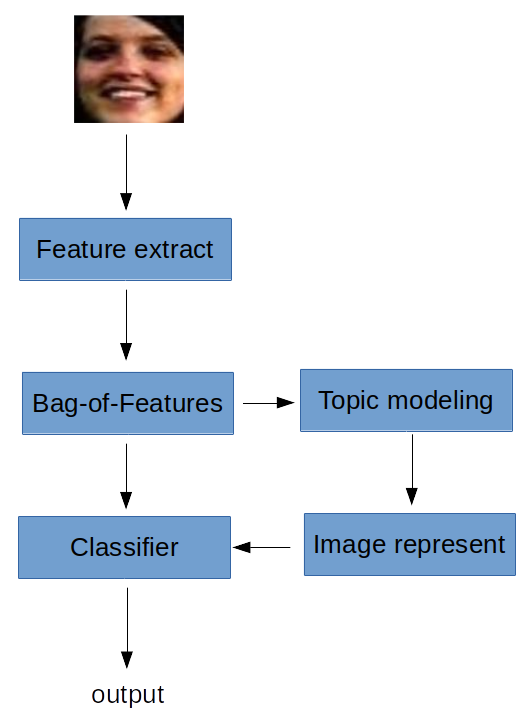
\includegraphics[width=.45\textwidth]{system-arch-cropped.png}
        \caption{System architect}
        \label{fig:system-architect}
    \end{figure}
\end{frame}

\section{Experiments and results}
\begin{frame}{Dataset - RAF-DB}
    \begin{table}[h!]
\centering
\caption{Number image in each class for training and testing} \label{tbl:raf-db-count}
\begin{tabular}{|l|c|c|}
\hline
\textbf{Class} & \textbf{Training} & \textbf{Testing} \\ \hline
Surprise & 1290 & 329 \\ \hline
Fear & 281 & 74 \\ \hline
Disgust & 717 & 160 \\ \hline
Happiness & 4772 & 1185 \\ \hline
Sadness & 1982 & 478 \\ \hline
Anger & 705 & 162 \\ \hline
Neutral & 2524 & 680 \\ \hline \hline
\textbf{Average} & \textbf{1753} & \textbf{438} \\ \hline
\textbf{Total} & \textbf{12271} & \textbf{3068} \\ \hline
\end{tabular}
\end{table}
\end{frame}

% \begin{frame}{Configure + ...}
    
% \end{frame}

\begin{frame}{Results - Bag-of-Words}
    \begin{table}[h!]
\centering
\caption{Bag-of-Words results, metric accuracy (\%)} \label{tbl:bag-of-words-metric}
\begin{tabular}{|l|l|l|}
\hline
Classifier & Unbalance & Balanced \\ \hline
NB & 41.82 & 30.02 \\ \hline
SVM & 49.0 & 40.64 \\ \hline
RF & 43.80 & 24.37 \\ \hline
\end{tabular}
\end{table}

\begin{figure} [h!]
    \centering
    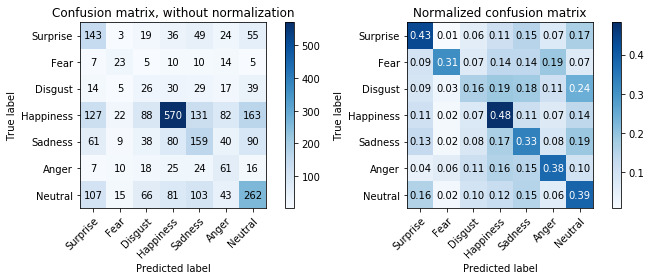
\includegraphics[width=.8\textwidth]{imgs/upsample-bow-svm.jpg}
    \caption{\tiny Bag-of-Words confusion matrix on balanced data with SVM}
    \label{fig:upsample-bow-svm}
\end{figure}

\end{frame}

\begin{frame}{Results - Topic modeling}
    \begin{table}[h!]
\centering
\caption{Topic modeling results, metric accuracy (\%)} \label{tbl:topic-modeling-metric}
\begin{tabular}{|l|l|l|}
\hline
Classifier & Unbalance & Balanced \\ \hline
NB & 39.89 & 22.90 \\ \hline
SVM & 40.12 & 22.35 \\ \hline
RF & 43.80 & 23.65 \\ \hline
\end{tabular}
\end{table}
\end{frame}

\begin{frame}{Discussion}
    % Please add the following required packages to your document preamble:
% \usepackage{multirow}
\begin{table}[]
\caption{Compare results} \label{tbl:topic-modeling-metric}
\begin{tabular}{|l|l|l|l|l|}
\hline
\multicolumn{1}{|c|}{\multirow{2}{*}{Classifier}} & \multicolumn{2}{c|}{Bag-of-Words} & \multicolumn{2}{c|}{Topic modeling} \\ \cline{2-5} 
\multicolumn{1}{|c|}{} & Unbalance & Balanced & Unbalance & Balanced \\ \hline
NB & 41.82 & 30.2 & 39.89 & 22.90 \\ \hline
SVM & 49.0 & 40.64 & 40.12 & 22.35 \\ \hline
RF & 43.80 & 24.37 & 43.80 & 23.65 \\ \hline
\end{tabular}
\end{table}
\end{frame}

% ---------------------------------
% SUMMARY
% ---------------------------------
% \section{Summary}
\begin{frame}{}
  \centering \Large
  \emph{Thank you!}
\end{frame}

%\ThankYouFrame

\end{document}
